%
%
% Header to use with branching.tex
%
% Used only to create a stand-alone branching.pdf

\documentclass[]{article}
\usepackage{natbib} % Bibliography
\bibpunct{(}{)}{;}{a}{}{;} % Bibliography
\setcitestyle{authoryear,open={},close={}} % Use 'It was found that something is something (Name 1234)' style

% Affiliations
\usepackage{authblk}
\title{Introduction}
\author[1]{Rich\`el J.C. Bilderbeek}
\affil[1]{Groningen Institute for Evolutionary Life Sciences, University of Groningen, Groningen, The Netherlands}


\usepackage{authblk}
\usepackage{booktabs}
\usepackage{siunitx} % handle units with proper spacing
\usepackage[final]{pdfpages} % add pdf pages
\usepackage{gensymb} % \degree symbol
\usepackage{afterpage} %page selection and control 
\usepackage{adjustbox} % Limit table
\usepackage{colortbl} % colors in tables.
\usepackage{rotating} % table rotation
\usepackage{microtype} % improves reading
\usepackage{textcomp} %fix apostrophes
\usepackage{textgreek}

\usepackage{listings}
\usepackage{hyperref}
\usepackage{todonotes}
\usepackage{verbatim}
\usepackage{pgf}
\usepackage{bm}

% Style of listings
% From http://r.789695.n4.nabble.com/How-to-nicely-display-R-code-with-the-LaTeX-package-listings-tp4648110.html
\usepackage{fancyvrb} 
\definecolor{codegreen}{rgb}{0,0.6,0}
\definecolor{codegray}{rgb}{0.5,0.5,0.5}
\definecolor{codepurple}{rgb}{0.58,0,0.82}
\definecolor{backcolor}{rgb}{0.95,0.95,0.92}
\lstdefinestyle{mystyle}{
  language=R,% set programming language
  basicstyle=\ttfamily\small,% basic font style
  commentstyle=\color{gray},% comment style
  % numbers=left,% display line numbers on the left side
  numberstyle=\scriptsize,% use small line numbers
  numbersep=10pt,% space between line numbers and code
  tabsize=2,% sizes of tabs
  showstringspaces=false,% do not replace spaces in strings by a certain character
  captionpos=b,% positioning of the caption below
  breaklines=true,% automatic line breaking
  escapeinside={(*}{*)},% escaping to LaTeX
  fancyvrb=true,% verbatim code is typset by listings
  extendedchars=false,% prohibit extended chars (chars of codes 128--255)
  alsoletter={.<-},% becomes a letter
  alsoother={$},% becomes other
  otherkeywords={!=, ~, $, \&, \%/\%, \%*\%, \%\%, <-, <<-, /},% other keywords
  deletekeywords={c}% remove keywords 
}
\lstset{style=mystyle}

% Use 'It was found that A is B (Name 1234)' style
\setcitestyle{authoryear,open={},close={}}

% To put figures 'Here'
\usepackage{float}

% subfigure
\usepackage{subfig}
\usepackage{graphicx}

% Need this, but needs to be installed
% \usepackage{multibib}

% TikZ drawing
\usetikzlibrary{arrows,automata}
\usetikzlibrary{calc}
\usetikzlibrary{arrows.meta}

\begin{document}

%%%%%%%%%%%%%%%%%%%%%%%%%%%%%%%%%%%%%%%%%%%%%%%%%%%%%%%%%%%%%%%%%%%%%%%%%%%%%%%%%%%%%%
% Figure 1
%%%%%%%%%%%%%%%%%%%%%%%%%%%%%%%%%%%%%%%%%%%%%%%%%%%%%%%%%%%%%%%%%%%%%%%%%%%%%%%%
\begin{figure}[H]
  \centering
  \resizebox {1.0\columnwidth} {!} {
    \begin{tikzpicture}[->,>=stealth',shorten >=1pt,auto,node distance=6cm, semithick]   
    \tikzstyle{every state}=[]
    \node[state] (A) [rectangle] {
      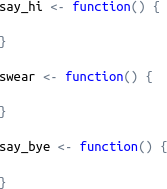
\includegraphics[width=0.2\textwidth]{1.png}
    };   
    \node[state] (B) [above right of = A, rectangle] {
      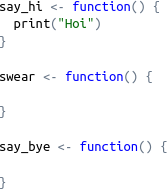
\includegraphics[width=0.2\textwidth]{2.png}
    };   
    \node[state] (C) [below right of = B, rectangle] {
      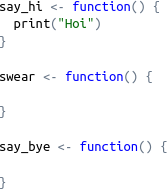
\includegraphics[width=0.2\textwidth]{2.png}
    };   
    \node[state] (D) [below right of = C, rectangle] {
      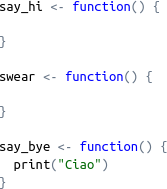
\includegraphics[width=0.2\textwidth]{3.png}
    };   
    \node[state] (E) [above right of = D, rectangle] {
      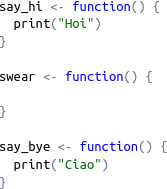
\includegraphics[width=0.2\textwidth]{4.png}
    };   
    \path 
      (A) edge [] node {} (B)
      (A) edge [] node {} (C)
      (B) edge [] node {} (C)
      (A) edge [] node {} (D)
      (C) edge [] node {} (E)
      (D) edge [] node {} (E)
    ; 
    \end{tikzpicture}
  }
\end{figure}
%%%%%%%%%%%%%%%%%%%%%%%%%%%%%%%%%%%%%%%%%%%%%%%%%%%%%%%%%%%%%%%%%%%%%%%%%%%%%%%%

%\newpage

%%%%%%%%%%%%%%%%%%%%%%%%%%%%%%%%%%%%%%%%%%%%%%%%%%%%%%%%%%%%%%%%%%%%%%%%%%%%%%%%%%%%%%
% Figure 1
%%%%%%%%%%%%%%%%%%%%%%%%%%%%%%%%%%%%%%%%%%%%%%%%%%%%%%%%%%%%%%%%%%%%%%%%%%%%%%%%
\begin{figure}[H]
  \centering
  \resizebox {1.0\columnwidth} {!} {
    \begin{tikzpicture}[->,>=stealth',shorten >=1pt,auto,node distance=6cm, semithick]   
    \tikzstyle{every state}=[]
    \node[state] (A) [rectangle] {
      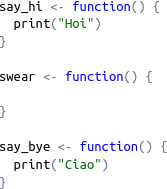
\includegraphics[width=0.15\textwidth]{4.png}
    };   
    \node[state] (B) [above right of = A, rectangle] {
      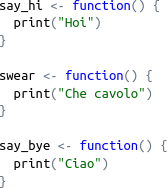
\includegraphics[width=0.15\textwidth]{5.png}
    };   
    \node[state] (C) [below right of = B, rectangle] {
      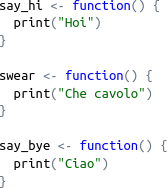
\includegraphics[width=0.15\textwidth]{5.png}
    };   
    \node[state] (D) [below right of = C, rectangle] {
      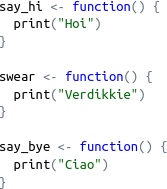
\includegraphics[width=0.15\textwidth]{6.png}
    };   
    \node[state] (E) [above right of = D, rectangle] {
      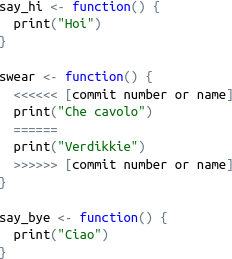
\includegraphics[width=0.15\textwidth]{7.png}
    };   
    \node[state] (F) [right of = E, rectangle] {
      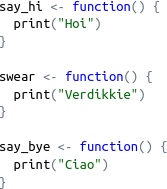
\includegraphics[width=0.15\textwidth]{8.png}
    };   
    \path 
      (A) edge [] node {} (B)
      (A) edge [] node {} (C)
      (B) edge [] node {} (C)
      (A) edge [] node {} (D)
      (C) edge [] node {} (E)
      (D) edge [] node {} (E)
      (E) edge [] node {} (F)
    ; 
    \end{tikzpicture}
  }
\end{figure}
%%%%%%%%%%%%%%%%%%%%%%%%%%%%%%%%%%%%%%%%%%%%%%%%%%%%%%%%%%%%%%%%%%%%%%%%%%%%%%%%



\end{document}
